\documentclass{article}
\usepackage{amsmath}
\usepackage{mathtools}
\usepackage{amsfonts}
\usepackage{amssymb}
\usepackage{amsthm}
\usepackage{fancyhdr}
\usepackage{float}
\usepackage{epigraph}
\usepackage{caption}
\usepackage{esint}

% Page formatting
\lhead{Eric Du}
\chead{Prelab 0}
\rhead{\today}
\pagestyle{fancy}
\cfoot{\thepage}
\title{Physics 5CL Prelab 0}
\author{Eric Du}
\date{\today}

%.sty file handling
\usepackage[sexy]{evan}
\usepackage{tcolorbox}
\usepackage{xcolor}
\renewcommand{\labelitemi}{\textendash}
\renewcommand{\abstractname}{}
\theoremstyle{definition}
\newtheorem*{solution}{\color{blue}Solution}
\numberwithin{equation}{section}
\numberwithin{definition}{section}

%Paragraph Formatting
\setlength{\epigraphwidth}{148pt}
\setlength{\parindent}{0pt}
\linespread{1.3}
\allowdisplaybreaks

%TikZ special settings
\usepackage{circuitikz}
\usetikzlibrary{patterns}
\usetikzlibrary{shapes.geometric}
\usetikzlibrary{decorations.markings}

\begin{document} 
\maketitle
\begin{abstract}
    \noindent \textbf{[NOTE:]} Although we have separate prelab submissions, I worked extensively with \textbf{Andrew Binder} to complete this prelab, so that is the reason why our work shares relatively similar styles.
\end{abstract}
\section*{Problem 1: Brick Geometry}

\textit{Consider the geometry of a ray of light incident on a rectangular brick of thickness t as shown. You may assume that the index of refraction of the surrounding air is 1.}

Refer to the following diagram for solutions, thanks to Andrew Binder for the TikZ: 

$$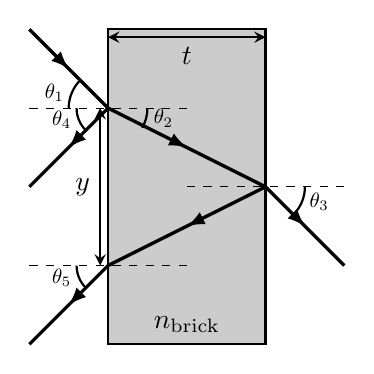
\begin{tikzpicture}
    [decoration={markings,
        mark= at position 0.5 with {\arrow{latex}}}
    ]
      \draw[thick,fill=gray!40] (0,0) -- (0,4) -- (2,4) -- (2,0) -- cycle;
      \draw[stealth-stealth,thick] (0,3.9) -- (2,3.9) node[midway,below]{$t$};
      \draw[postaction={decorate},very thick] (-1,4) -- (0,3);
      \draw[dashed] (-1,3) -- (1,3);
      \draw[postaction={decorate},very thick] (0,3) -- (-1,2);
      \draw[postaction={decorate},very thick] (0,3) -- (2,2);
      \draw[dashed] (1,2) -- (3,2);
      \draw[postaction={decorate},very thick] (2,2) -- (3,1);
      \draw[postaction={decorate},very thick] (2,2) -- (0,1);
      \draw[dashed] (-1,1) -- (1,1);
      \draw[postaction={decorate},very thick] (0,1) -- (-1,0);
      \node at (1,0.25) (n) {$n_{\text{brick}}$};
      \draw[stealth-stealth,thick] (-0.1,3) -- (-0.1,1) node[midway,left] {$y$};
      \draw[thick] (-0.5,3) arc (180:135:0.5cm) node[midway,left,scale=0.75] {$\theta_1$};
      \draw[thick] (0.5,3) arc (0:-30:0.5cm) node[midway,right,scale=0.75] {$\theta_2$};
      \draw[thick] (2.5,2) arc (0:-45:0.5cm) node[midway,right,scale=0.75] {$\theta_3$};
      \draw[thick] (-0.4,3) arc (180:225:0.4cm) node[midway,left,scale=0.75] {$\theta_4$};
      \draw[thick] (-0.4,1) arc (180:225:0.4cm) node[midway,left,scale=0.75] {$\theta_5$};
    \end{tikzpicture}$$


\begin{enumerate}[a)]
\item \textit{Determine $z$ in terms of the lengths $t$ and $y$ (you just need geometry for this part - no Snell's law is allowed)}

Purely from geometry, we get

\[ z = \sin \theta_2 = \frac{\frac{y}{2}}{\sqrt{\left(\frac{y}{2}\right)^2 + t^2}}\]

\item \textit{Use propagation of errors to determine $\alpha_x$ as a function of $\theta_1$ and $\alpha_{\theta_1}$. Then determine $\alpha_z$ as a function of $t, y,\alpha_t$ and $\alpha_y$.} 

We have:

\[ \alpha_Z = \sqrt{\left(\frac{\partial z}{\partial y} \alpha_y\right)^2 + \left(\frac{\partial z}{\partial t} \alpha_t\right)^2}\]

Thus, computing the partial derivative separately:

\begin{align*}
    \frac{\partial z}{\partial y} &= \frac{1}{2}\left(\frac{\sqrt{\frac{y^2}{4} + t^2} + \frac{y}{2\left(\frac{y^2}{4} + t^2\right)^{1/2}}}{\left(\frac{y}{2}\right)^2 + t^2}\right)\\
    \frac{\partial z}{\partial t} &= \frac{y}{2} \cdot \frac{1}{\left[\left(\frac{y}{2}\right)^2 + t^2\right]^{3/2}} \cdot -\frac{1}{2}(2t)\\
    \therefore \alpha_z &= \left[\left(\frac{\alpha_y}{2}\left(\frac{\sqrt{\frac{y^2}{4} + t^2} + \frac{y}{2\left(\frac{y^2}{4} + t^2\right)^{1/2}}}{\frac{y^2}{4} + t^2}\right)\right)^2 + \left(\frac{yt}{2\left[ \frac{y^2}{4} + t^2\right]^{3/2}} \alpha_t \right)^2 \right]^{1/2}
\end{align*}

\item \textit{Show that the geometry of reflection and refraction implies that $\theta_1 = \theta_3 = \theta_4 = \theta_5$}

By the law of reflection, the angle of incidence equals the angle of reflection, and thus $\theta_1 = \theta_4$. From Snell's law, we have $\sin{\theta 1} = n \sin \theta_2$ and $n \sin \theta_2 = \sin{\theta_3}$, so $\sin \theta_1 = \sin \theta_3 \implies \theta_1 = \theta_3$. This is also true because all $\theta < 90$ due to the way we interpret the angles, so there is only one unique soluiton to $\sin \theta_1 = \sin \theta_3$.

Further, by parallel lines we get $n \sin \theta_2 = \sin \theta_5 = \sin \theta_1$, so this leads to $\theta_1 = \theta_5$, and thus $\theta_1 = \theta_3 = \theta_4 = \theta_5$.


\item \textit{Use Snell's law and your result from (a) to determine the index of refraction of the brick $n_{brick}$ first in terms of $x$ and $z$ and then in terms of $t, y$ and $\theta_1$.}

From Snell's law earlier, we had $n \sin \theta_2 = \sin \theta_1$, so we have:

\[ n = \frac{\sin \theta_1}{\sin\theta_2} = \frac{x}{z}\]

To express this in terms of $t, y$ and $\theta_1$:

\[ n = \frac{\sin\theta_1}{\frac{y/2}{\sqrt{\frac{y^2}{4} + t^2}}} = \frac{2\sin \theta_1 \sqrt{\frac{y^2}{4} + t^2}}{y}\]


\item \textit{Perform a propagation of errors to determine the uncertainty in $n_{brick}$ based on the uncertainties of $\alpha_x$ and $\alpha_z$.}

Since $n = \frac{x}{z}$, the error propagation is as follows: 

\begin{align*} 
    \alpha_n &= \sqrt{\left(\frac{-x}{z^2}\alpha_z\right)^2 + \left(\frac{1}{z} \alpha_x\right)^2}\\
    &= \frac{1}{z} \sqrt{\frac{x^2}{z^2}\alpha_z^2+ \alpha_x^2}
\end{align*}
\end{enumerate}

\section*{Problem 2: Least-Squares with Hypothesis $y = -x + b$}

\textit{Consider the hypothesis $y = -x + b$. The function $\chi^2$ for a \textbf{weighted} least squares analysis is }

\[ \chi^2 = \sum w_i(y_i + x_i - b)^2 = \sum \left(\frac{y_i +x_i - b^2}{\alpha_{y, equiv, i}}\right)^2\]

\textit{where $\alpha_{y, equiv, i}$ is given by $\sqrt{\alpha_{yi}^2 + \alpha_{xi}^2}$}


\begin{enumerate}
    \item \textit{Find the best fit value $b$ which minimizes $\chi^2$. You may use the weights $w_i$ in your answer as we did in Eqs. 5.3.1 and 5.3.3-5.3.5 in the Statistics Review Sheet}
    

    From equation 5.4.5b on the statistics review sheet, we have 

    \[ b = \frac{\sum w_i y_i - m \sum w_i x_i}{\sum w_i}\]

    And since our model is $y = -x + b$, we have $m = -1$ so:

    \[ b = \frac{\sum w_i y_i + \sum w_ix_i}{\sum w_i}\]


    \item \textit{Use propagation of errors on your answer from (a) to determine the error in your best fit value $\alpha_b$. Hint: Use the trick of shifting all the errors from $x$ over to $y$, so $\delta x_i = 0$ and $\delta y_i = \delta y_{equiv, i}$(You may use the weights $w_i$ in your answer.)}
    
    Following the hint, we assume that $\delta x_i = 0$, and so all errors are in $\delta y_i$. For this specific formula, the error propagation is: 
    
    \[ \alpha_b = \sqrt{\sum \left(\frac{\partial b}{\partial y_i} \alpha y_i\right)^2} = \sqrt{\sum \left(\frac{w_i}{\sum w_i} \alpha_{yi}\right)^2} = \sqrt{\frac{(\sum w_i \alpha_{yi})^2}{(\sum w_i)^2}}\]

\pagebreak

\section*{Part 3: Laser Safety}

Here's the screenshot for laser safety:

\begin{center}
    \includegraphics[scale=0.5]{laser safety.png}
\end{center}

\end{enumerate}
\end{document}
